% !TEX root = ../thesis.tex
\chapter{Context-Aware Data Mashups: Approach}
\label{capitolo4}
\thispagestyle{empty}
In this chapter, we will be discussing and justifying our design decisions, and we will provide a description of the high-level architecture of our system. As previously stated, our work will focus on the backend component, which takes care of service querying and data integration.\\
\section{Design Decisions}
\subsection{Service Querying with PerLa}
PerLa\footnote{http://perla.dei.polimi.it/middleware.php}\cite{perla} is a middleware technology developed in Politecnico di Milano. The main aim of this middleware at the time was to query pervasive systems that exist in a heterogeneous environment, and provide a homogenous abstraction of the different devices that make up this system. In CAMUS, part of the system is going to have query different web services, and provide an abstract homogenous interface that contains the results of these queries. Therefore, using PerLa as a tool to provide such abstraction was a reasonable option.\\\\
The way PerLa works is as follows: the first step is to generate (or manually write) an XML descriptor for each device in the pervasive system. Since different sensors often have different structures for their replies, the descriptor's job is to allow PerLa to know what to expect. The descriptor specifies what the structure of the reply is, as well as some other factors, such as the protocol used for communication (i.e. http, https etc...), the request method (GET, POST etc...), and the destination URL of the request. The descriptor also includes details on which response elements are interesting to us, so that we can retrieve and query for them. Finally, we can include at the end of the XML file any post-processing we want to do, in terms of editing the content of the response, using the PerLa scripting language.\\\\
In theory, we can adapt PerLa and use it to query REST APIs instead of pervasive systems. In this case, the web services are similar to the sensors that we were querying in the case of pervasive systems. Moreover, the descriptors would describe these web services (request parameters, response format etc...), in a similar way to how they used to describe the sensors.\\\\ Unfortunately, PerLa requires performing some complex steps to set up, before we could use it for REST APIs. As we prepared PerLa for the needed tasks, we started figuring out the missing components and performing the necessary adjustments. In particular, PerLa did not natively support including HTTP headers when sending requests. Therefore, we had to locate the area in the code where the requests were being built and sent, and then we added the required code to support adding headers to requests.

\begin{lstlisting}
getRequest = new HttpGet(request.getUri());
String head = request.getHeaders();
if (head != null && !head.equals("")) {
	String[] headers = head.split(";");
	for (int i = 0; i < headers.length; i++) {
		String[] header = headers[i].split(":");
		getRequest.addHeader(header[0], header[1]);
	}
}
\end{lstlisting}

\noindent This code allows adding headers to the XML descriptor of the web service as follows: in the requests object, we add an attribute ``headers'', and assign to it the header as key:value. With this code, we can also add multiple headers, and we separate the different key-value pairs using semicolons. We also edited other various areas in the code to make this code work, as building the HTTP request goes through multiple phases in different Java classes.\\\\
Preliminary results with PerLa seemed promising: we were able to adapt this stable, solid framework to our needs. We performed these tests manually by writing XML descriptors for simple services (mostly weather services) because the responses were simple enough, and mapping them to XML was not too challenging. Naturally, we also want our code to work with more complex responses, as this is the case for most modern APIs. Modern APIs return responses that include multiple objects of various structured, nested arrays, and such structures are not simple when it comes to mapping them to XML descriptors for PerLa.\\\\
For this reason, the next step we decided to work on is finding a way to automatically generate an XML descriptor for each web service, based on the JSON responses returned by the service. The descriptor generator should be able to parse the response, figure out the schema of this response regardless of the actual data context returned, and output an XML descriptor that we would directly plug into PerLa. In this way, this descriptor should work with any response returned by that specific API endpoint, for any values of the query parameters we include when querying the service.\\\\
After doing some research, we found that there are many libraries written in various languages that can generate a JSON Schema-like structure for any JSON document. This was interesting because mapping a JSON schema to an XML schema is much simpler than mapping a JSON response to an XML schema. Thus, by using such libraries, we would already be half-way on the path of generating the XML schema that PerLa requires. We ended up using a Jskemator, a public Python library available on Github. This library did its job perfectly well, and the next step would be to add the code needed to map JSON schema to XML schema. We wrote the corresponding code in Python as well, and as we tried it on different web services, we started figuring out some particularities in the way PerLa parses the XML descriptors. Specifically, when generating the response schema, we should define the different objects in a bottom-up approach. This means that in the case of nested objects, for example, we should define the innermost object first, and then progressively go outwards until we reach the top level. At first sight, this does not seem very complicated, and all we have to do is keep track of the current nesting level we have reached, and then re-order all the structures we have generated based on the nesting order. After testing with many services, we realized that it is not easy to solve this issue, for the reasons mentioned in the following point.\\\\
The second point we noticed is that PerLa in its current implementation does not support the presence of multiple objects sharing the same ID in the same JSON response. Therefore, even if the original response contains such objects, and in case they do not share the same structure, our code must somehow make the IDs in the corresponding XML schema distinct. However, this proved to be more difficult when querying some of the more complex services we mentioned. Taking Foursquare as an example, the response contains several nested objects that share the same IDs as the parent objects (sometimes several levels going up), and this created the problem of circular dependency, as we ended up with the inner objects being dependent on the outer ones.\\\\
The third issue we ran into was when we realized that, since the URL we are querying is hard-coded in the descriptor, we needed to create a different XML file not only for each service we query, but also for each query to the same service any time we change the value of a query parameter. This is a problem because, in a real life scenario, we will be querying the services multiple times, with different parameters, and having to create a separate descriptor for each query renders using PerLa unfeasible. Another important drawback of PerLa is that, after querying different services, we will need to perform joins in order to integrate the different responses into one logical group, and such operations are not natively supported by PerLa. Therefore, we would anyway need to use an external DBMS or module to accomplish this task.\\\\
Finally yet importantly, PerLa supports querying multiple services simultaneously. However, in case the services share objects that have the same name, PerLa does not support choosing which service to query for this object. This is yet another thing that we will have to add to the core code of PerLa. After doing these tests and realizing the shortcomings of PerLa, we opted not to use it, since the work we will need to do in order to add the needed features will be very time-consuming, and this outweighs the advantages of using a this well-established framework. In the end, we decided to perform simply the queries to the services manually using any programming language of our choice, therefore bypassing the need to upgrade PerLa to have it satisfy our requirements.
\newpage
\section{Architecture}
\label{sec:architecture}
After making sure that in its current state, PerLa does not satisfy our needs, we decided to move forward without including it as a component in the CAMUS system. Therefore, we now had complete freedom in choosing the language in which to implement the different components we need. We opted to use PHP to send the requests and parse the responses. Next, we had to find numerous free APIs belonging to a specific category, and these APIs must fit within the Travel Agent scenario. This was quite a difficult task because there aren't many public free APIs that provide a generic search functionality and go well with the proposed scenario. Fortunately, in the end we were able to find three APIs that allow searching for events in a specific location (PredictHQ, Ticketmaster, Eventful, Eventbrite), and three APIs that lists restaurants also given a location (Zomato, Yelp, Foursquare). This makes sense in terms of travelling activities because tourists are usually interested in both finding places to eat and events to attend. This also was interesting because it opens the possibility of performing joins between these two categories, e.g. searching for sushi restaurants that are located around a certain event.\\\\
After choosing these seven sample APIs, we wrote the code needed to query each of them, and proceeded to study the differences in the way each of them expects a request and provides a reply. Naturally, different APIs both require differently formed requests, and respond in variously structured formats. For instance, some APIs require header authentication, while others perform authentication using URL parameters.\\\\
Figure 4.1 shows the high-level architecture of the backend component, and we will elaborate on the role of each part in the following parts.
\newpage
\begin{figure}[h]
\centering
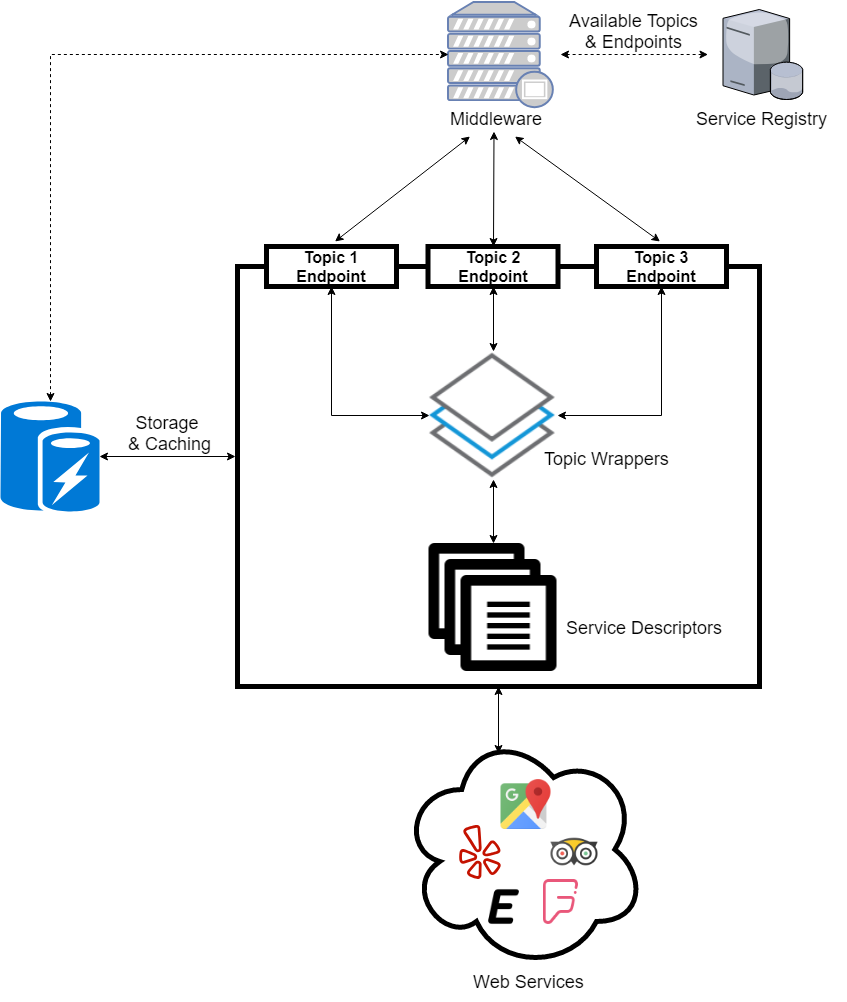
\includegraphics[width=\textwidth]{genarch}
\caption{High-Level Architecture View}
\end{figure}
\newpage
\subsection{Wrapper Approach}
The next step was to write code that is generic enough, allowing it to be easily adapted to any additional APIs we decide to add later on. Therefore, we decided to implement the concept of wrappers to achieve this task. In the book ``Principles of Data Integration'', Doan et al.\cite{doan} state that a wrapper is the medium that communicates with data sources by sending them requests and then parsing the corresponding responses, usually converting these responses to a unified homogeneous format. A wrapper's complexity varies greatly, depending on the data sources that it interfaces with. For instance, a wrapper would be relatively simple to construct if its purpose is to integrate two or more databases, since the mapping between the structures in these databases is static. Therefore, all that is required is to define the elements of interest, and how to extract them from the respective databases (i.e. where to find them, table name, column name and so on).\\\\
This process becomes more complicated when dealing with web services: the replies returned by web services usually differ greatly in structure, and even within the scope of one service, the reply structure might also depend on the request parameters that were initially sent. Therefore, a wrapper for web services should be able to dynamically accommodate for such variations, and still find the relevant information within the received replies.\\\\
Therefore, we needed to create a generic wrapper that is able to receive a request from the middleware, and using the service descriptors, adapt this generic request so that it can be sent to each of the relevant web services, thereby transforming the resource schema-based requests into service-specific requests. Then, the wrapper extracts the relevant information from the replies received from the web services, and integrates the resulting outputs into one structure that is based on the resource schema. Finally, this end result is finally sent back to the middleware. This process is illustrated in figure 4.2.
\begin{figure}[h]
\centering
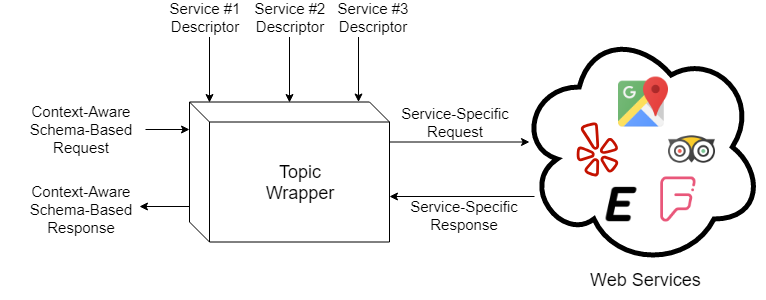
\includegraphics[width=\textwidth]{wrapper}
\caption{Service Wrapper}
\end{figure}
\newpage
\noindent In order to implement this functionality, we defined the structure of the objects we are querying for (i.e. restaurants and events), specified the fields that interest us, and defined the corresponding classes along with their constructors. The aim here is to extract the information we need from various APIs, and then use the constructors of these classes in order to create a homogenous array of objects that contains this information.\\\\
Sticking with the idea that we want our code to be generic and devoid of any service-specific details, we decided to include such details in external JSON files (descriptors). When needed, these files will be parsed in order to identify how to query said services, and what parameters to include in the requests.\\\\
The following figure shows a skeleton of a JSON service descriptor. The role of each object included in a JSON descriptor will be explained later on, but the point behind these descriptors is to supply the wrapper with knowlege on how to query the services, what parameters they expect, and how to parse their responses.
\newpage
\begin{figure}[h]
\centering
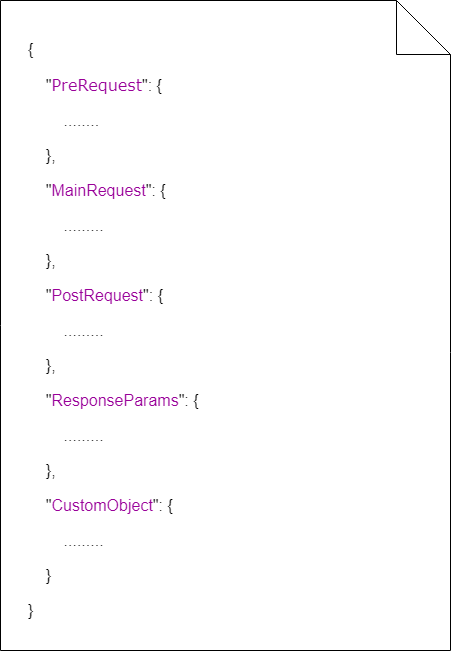
\includegraphics[scale=0.49]{descriptor}
\caption{Service Descriptor Skeleton}
\end{figure}
\noindent Since the middleware is the component that creates and sends the inital request, we have to provide a way for the middleware to know what kind of resources are available, what are the required request parameters for each available API, as well as the structure of the response that the backend will generate, so that the middleware can parse these responses. To that, the ListServices API was created, and the response of this API is a list of all of the available services, along with the relevant details. The following is a sample response, containing only two services (restaurants and events). Whenever new services are added, a corresponding description should be added to this API's response.
\newpage
\begin{lstlisting}[language=json,firstnumber=1]
{
  "restaurants": {
    "endpoint": "GETRestaurants.php",
    "params": {
      "city": "string",
      "query": "string",
      "lon": "float",
      "lat": "float"
    },
    "attributes": {
      "name": "string",
      "address": "string",
      "url": "string",
      "latitude": "float",
      "longitude": "float",
      "geohash": "string",
      "cusisines": "string",
      "thumb": "string",
      "phone": "string",
      "rating": "float"
    }
  },
  "events": {
    ...
  },
  "news": {
    ...
  },
  "weather": {
    ...
  }
}
\end{lstlisting}
\pagebreak
\subsection{Storage and Caching}
After we developed a working system that can send requests to multiple services and integrate their responses, a testing phase took place in order to study the efficiency of this system and find ways to improve it. Right away, we noticed that querying multiple services and doing all of pre- and post-processing is a costly operation, especially in terms of running time. For instance, querying for music events that are taking place in Boston had an average running time of 30 seconds, during which we queried four different related APIs and performed all the necessary operations to integrate their responses. From a regular user's perspective, 30 seconds is a long wait for such a simple query, especially in the case where they want to perform multiple searches with different keywords.\\\\
To mediate this drawback, we decided to add caching functionalities, thus reducing the amount of requests we send out to the various web services. The caching will be done as shown in the following figure:
\begin{figure}[h]
\centering
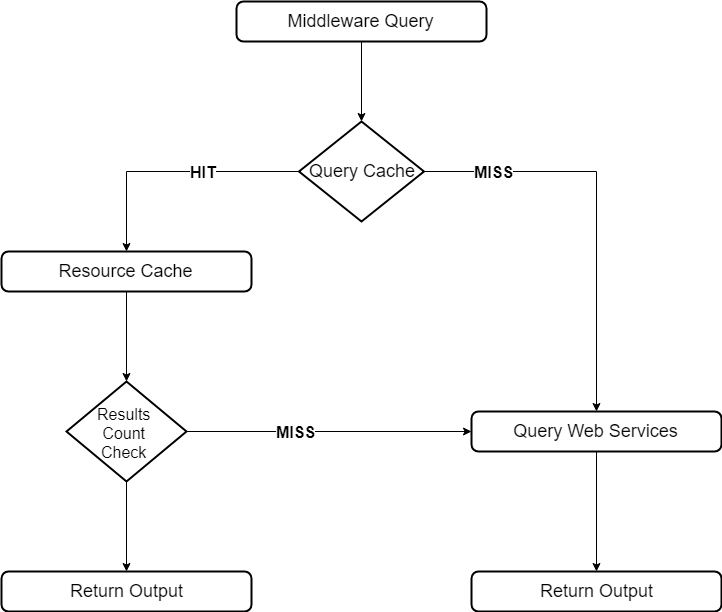
\includegraphics[scale=0.46]{cachediagram}
\caption{Caching Schema}
\end{figure}
\newpage
\noindent The caching is done in two phases: at query time and at response time. The first phase, query caching, consists of saving the information related to every query that is received from the middleware. Query caching allows us to check whether a query similar to one that we are about to send now has already been issued within a certain (recent) timeframe. In case the cache check results in a miss, that means that no similar query has been issued recently, and therefore we must query the web services to retrieve the requested information. However, it is worthy to note that as the system scales and the number of users increases, the number of instances where the query cache will result in a miss should decrease noticeably.\\\\
In case the query cache check results in a hit, we can safely assume that a similar query has been sent. This is where the second phase of caching comes into play: it consists of saving the output of responses we receive when querying the web services. The information we store in the cache matches the structure of the resource schema, and this means that no further processing is needed whenever we query for this data later on.\\\\
The outcome of this process is a reduction in the number of requests we issue to the web services, which reduces the running time a lot since this is the actual bottleneck in our operation flow. Nonetheless, we still have to make sure that the cardinality of the response resulting from querying the second level of cache is above the required threshold. If that is not the case, we have to fall back again to querying the web services in order to update the resource cache with new data and refresh what already exists as well.